\documentclass[conference]{IEEEtran}

\IEEEoverridecommandlockouts
% The preceding line is only needed to identify funding in the first footnote. If that is unneeded, please comment it out.
\usepackage{cite}
\usepackage{amsmath,amssymb,amsfonts}
\usepackage{booktabs}
\usepackage{algorithmic}
\usepackage{graphicx}
\usepackage{adjustbox}
\usepackage[inline]{enumitem}
\usepackage{textcomp}
\usepackage{lipsum}
\usepackage{xcolor}
\usepackage{tikz}
\usepackage{float}
\usepackage{placeins}
\usepackage{listings}
\usepackage{pifont}
\PassOptionsToPackage{hyphens}{url}\usepackage{hyperref}
\usepackage{cleveref}
\setlength{\marginparwidth}{2cm}
\usepackage[colorinlistoftodos,prependcaption,textsize=tiny]{todonotes} % \usepackage[colorinlistoftodos,prependcaption,textsize=tiny]{todonotes} to disable the notes
\usepackage{xargs}                    
\newcommand{\todocite}[1]{\todo[color=green!40]{#1}}
\usepackage{tabularray}
\usepackage{pifont}
\usepackage{tabularx}

\usepackage[T1]{fontenc}
\usepackage[scaled=0.85]{inconsolata} % optional mono font
\usepackage{xcolor}

\definecolor{KeywordBlue}{RGB}{0,92,197}
\definecolor{OpRed}{RGB}{178,34,34}
\definecolor{NumTeal}{RGB}{0,128,128}
\definecolor{CommentGray}{gray}{0.35}

\crefname{listing}{Listing}{Listings} % enables \Cref{<label>} for listings
\lstdefinestyle{pyopendt}{
  language=Python,
  basicstyle=\ttfamily\small,
  frame=single,
  breaklines=true,
  breakatwhitespace=true,
  showstringspaces=false,
  columns=fullflexible,
  % keep strings black
  stringstyle=\color{black},
  commentstyle=\color{CommentGray},
  keywordstyle=\color{KeywordBlue},
  % emphasize selected identifiers (pseudo-builtins in your snippet)
  emph={json,parser,sim_results,batch_data,current_topology,slo_targets},
  emphstyle=\color{KeywordBlue},
  % color operators, braces, punctuation, and digits
  literate=
   *{+}{{{\color{OpRed}+}}}1
    {-}{{{\color{OpRed}-}}}1
    {*}{{{\color{OpRed}*}}}1
    {/}{{{\color{OpRed}/}}}1
    {=}{{{\color{OpRed}=}}}1
    {:}{{{\color{OpRed}:}}}1
    {,}{{{\color{OpRed},}}}1
    {(}{{{\color{OpRed}(}}}1
    {)}{{{\color{OpRed})}}}1
    {[}{{{\color{OpRed}[}}}1
    {]}{{{\color{OpRed}]}}}1
    {.}{{{\color{OpRed}.}}}1
    {0}{{{\color{NumTeal}0}}}1
    {1}{{{\color{NumTeal}1}}}1
    {2}{{{\color{NumTeal}2}}}1
    {3}{{{\color{NumTeal}3}}}1
    {4}{{{\color{NumTeal}4}}}1
    {5}{{{\color{NumTeal}5}}}1
    {6}{{{\color{NumTeal}6}}}1
    {7}{{{\color{NumTeal}7}}}1
    {8}{{{\color{NumTeal}8}}}1
    {9}{{{\color{NumTeal}9}}}1
}

\newcommand\blfootnote[1]{%
  \begingroup
  \renewcommand\thefootnote{}\footnote{#1}%
  \addtocounter{footnote}{-1}%
  \endgroup
}

\newcommandx{\todolarge}[2][1=]{\todo[inline,size=\large,linecolor=blue,backgroundcolor=cyan,bordercolor=blue,#1]{#2}}
\newcommand{\todoother}[1]{\todo[inline, color=cyan!40]{Other: #1}}
\newcommand{\todoall}[1]{\todo[inline, color=orange!40]{TODO: #1}}
\newcommand{\todoradu}[1]{\todo[inline,color=teal!40]{Radu: #1}}
\newcommand{\todoalexis}[1]{\todo[inline, color=gray!40]{Alexis: #1}}
\newcommand{\todomahesh}[1]{\todo[inline, color=green!40]{Mahesh: #1}}
\newcommand{\todoben}[1]{\todo[inline, color=purple!40]{Ben: #1}}



% Citation own system
\newcommand{\citationstodo}[1]{\textsuperscript{\color{blue} [#1]}}
% Citation needed
\newcommand{\citationneeded}{\textsuperscript{\color{blue} [citation needed]}}
\newcommand{\citationsneeded}[1]{\textsuperscript{\color{blue} [#1 needed]}}


%%% \verify, \cut, \addref, \unsure, \change, \info, \improvement, \thiswillnotshow
\newcommand{\verify}[1]{\todo[inline, color=cyan!40]{check: #1}}
\newcommand{\cut}[1]{\todo[inline, color=yellow!40,disable]{Cut: #1}}
\newcommandx{\addref}[2][1=]
{\todo[inline,linecolor=blue,backgroundcolor=blue!50,bordercolor=blue,#1]{Add reference. #2}}
\newcommandx{\unsure}[2][1=]{\todo[inline, linecolor=red,backgroundcolor=red!25,bordercolor=red,#1]{#2}}
\newcommandx{\change}[2][1=]{\todo[inline, linecolor=blue,backgroundcolor=blue!25,bordercolor=blue,#1]{#2}}
\newcommandx{\info}[2][1=]{\todo[linecolor=OwnOliveGreen,backgroundcolor=OwnOliveGreen!25,bordercolor=OwnOliveGreen,#1]{#2}}
\newcommandx{\improvement}[2][1=]{\todo[linecolor=Plum,backgroundcolor=Plum!25,bordercolor=Plum,#1]{#2}}
\newcommandx{\thiswillnotshow}[2][1=]{\todo[disable,#1]{#2}}
%

\definecolor{darkred}{rgb}{0.5,0,0}
\definecolor{darkgreen}{rgb}{0,0.5,0}
\definecolor{darkblue}{rgb}{0,0,0.5}
\newcommand{\note}[1]{\noindent\textbf{\textsc{\textcolor{darkgreen} {(NOTE: #1)}}}}
\newcommand{\NOTE}[1]{\noindent\textbf{\textsc{\textcolor{red} {(IMPORTANT: #1)}}}}

\newcommand{\circled}[1]{%
    \tikz[baseline=(char.base)]{
        \node[shape=circle, fill=black, text=white, inner sep=0.5pt, font=\small] (char) {#1};
    }%
}


\def\BibTeX{{\rm B\kern-.05em{\sc i\kern-.025em b}\kern-.08em
    T\kern-.1667em\lower.7ex\hbox{E}\kern-.125emX}}

\makeatletter
\setlength{\@fptop}{0pt}
\makeatother

\begin{document}

\newpage
\title{OpenDT: \underline{Open}-source \underline{D}igital \underline{T}winning Instrument for Monitoring and Operating Datacenters}

% How to design, implement, and evaluate an integrated system for digital twinning performance and sustainability of datacenters?
\author{
\IEEEauthorblockN{Radu Nicolae\textsuperscript{*}, Gleb Mishchenko\textsuperscript{*}, Isidora Jovanović\textsuperscript{*}, Domas Davidavicius\textsuperscript{*}, Martin Oltmann\textsuperscript{*} } 
\IEEEauthorblockA{\textit{Vrije Universiteit Amsterdam} \\
Amsterdam, The Netherlands \\
\{r.nicolae, g.mishchenko, i.jovanovic2, d.davidavicius, m.g.oltmann\}@student.vu.nl}
}





% \makeatletter
% \newcommand{\linebreakand}{%
%   \end{@IEEEauthorhalign}
%   \hfill\mbox{}\par
%   \mbox{}\hfill\begin{@IEEEauthorhalign}
% }
% \makeatother

% \author{
% \IEEEauthorblockN{Radu Nicolae*}
% \IEEEauthorblockA{\textit{Vrije Universiteit Amsterdam} \\
% Amsterdam, The Netherlands \\
% r.nicolae@student.vu.nl}
% \and
% \IEEEauthorblockN{Gleb Mishchenko*}
% \IEEEauthorblockA{\textit{Vrije Universiteit Amsterdam} \\
% Amsterdam, The Netherlands \\
% d.niewenhuis@vu.nl}
% \and
% \IEEEauthorblockN{Isidora Jovanović*}
% \IEEEauthorblockA{\textit{Vrije Universiteit Amsterdam} \\
% Amsterdam, The Netherlands \\
% s.talluri@vu.nl}
% \linebreakand
% \IEEEauthorblockN{Domas Davidavicius*}
% \IEEEauthorblockA{\textit{Vrije Universiteit Amsterdam} \\
% Amsterdam, The Netherlands \\
% a.iosup@vu.nl}
% \and
% \IEEEauthorblockN{Martin Oltmann*}
% \IEEEauthorblockA{\textit{Vrije Universiteit Amsterdam} \\
% Amsterdam, The Netherlands \\
% a.iosup@vu.nl}
% \thanks{*All authors contributed equally to this work.}
% }


% \makeatletter
% \newcommand{\newlineauthors}{%
%   \end{@IEEEauthorhalign}\hfill\mbox{}\par
%   \mbox{}\hfill\begin{@IEEEauthorhalign}
% }
% \makeatother

% \author{
% \IEEEauthorblockN{Radu Nicolae}
% \IEEEauthorblockA{\textit{Vrije Universiteit Amsterdam} \\
% Amsterdam, The Netherlands \\
% r.nicolae@student.vu.nl}
% \and
% \IEEEauthorblockN{Gleb Mishchenko}
% \IEEEauthorblockA{\textit{Vrije Universiteit Amsterdam} \\
% Amsterdam, The Netherlands \\
% d.niewenhuis@vu.nl}
% \and
% \IEEEauthorblockN{Isidora Jovanović}
% \IEEEauthorblockA{\textit{Vrije Universiteit Amsterdam} \\
% Amsterdam, The Netherlands \\
% s.talluri@vu.nl}

% \vspace{-1cm}
% \newlineauthors

% \IEEEauthorblockN{Domas Davidavicius}
% \IEEEauthorblockA{\textit{Vrije Universiteit Amsterdam} \\
% Amsterdam, The Netherlands \\
% a.iosup@vu.nl}
% \and
% \IEEEauthorblockN{Martin Oltmann}
% \IEEEauthorblockA{\textit{Vrije Universiteit Amsterdam} \\
% Amsterdam, The Netherlands \\
% a.iosup@vu.nl}

% \vspace{-3cm}
% }




\maketitle
\thispagestyle{plain}
\pagestyle{plain}



\begin{abstract}
Datacenters represent the backbone of our digital society, but raise operational challenges when workload grows.
We envision digital twins as becoming primary instruments in datacenter operation, continuously and autonomously adapting ICT infrastructure on demand with a human-in-the-loop for major decisions.
However, unlike other fields that successfully employ digital twins (e.g., aviation, autonomous driving), and albeit its critical importance in ICT operation, a digital twinning ecosystem for operating and monitoring ICT infrastructure has never been proposed.
Addressing this challenge, we propose \underline{OpenDT}, the first \underline{Open}-source, \underline{D}igital \underline{T}winning Ecoystem for monitoring and operating datacenters through a continuous integration cycle:
(1) live and continuous telemetry data;
(2) discrete-event simulation using a digital twin of the physical ICT infrastructure, adapted to the live telemetry data, and evaluated against Service Level Objectives (SLOs);
(3) LLM-based, and human-approved feedback to physical ICT; and
(4) adjustment of the phyiscal ICT following the feedback.
In this work, our contribution is twofold: firstly, we propose a high-level design of OpenDT against established functional and non-functional requirements; secondly, adhering to state-of-the-art practices, we engineer a prototype of OpenDT.
\end{abstract}

% The framework for digital twinning ICT ecosystems in the Nethelands has been set by AtLarge Team ... A reference architecture has been proposed and developed by the AtLarge Research Team and partners in the Groeifonds programma 6G FNS.

% This project is the first to set up ...

% 1) Unseen OpenDC Scenarios
% 2) LLMs in scenario/topology, and data extraction. LLMs that make the input info structured and sets up the simulator
% 3) Multi-Model simulation in the simulation component

\begin{IEEEkeywords}
datacenters, digital twins, simulation, performance, energy utilization, OpenDT
\end{IEEEkeywords}


 % Datacenters represent the backbone of our digital society, but raise operational challenges when workload grows. 
  % We envision digital twins as becoming primary decision-making instruments for datacenter operation, continuously adapting infrastructure on demand following a human-in-the-loop paradigm.
  % However, unlike other fields that successfully employ digital twins (e.g., aviation, autonomous car driving), it has never been proposed a digital twinning system of ICT infrastructure under workload. 
  % Addressing this challenge, we propose \underline{OpenDT}, the first \underline{Open}-source, end-to-end, workload-aware \underline{D}igital \underline{T}winning System for monitoring and operating datacenters designed with a continous integration cycle: 
  % (1) live and continuous telemetry data, 
  % (2) discrete-event simulation using as input a digital twin of the physical ICT infrastructure, telemetry data, and defined Service Level Objectives (SLOs), 
  % (3) feedback to the physical ICT, and 
  % (4) adjustment of the physical infrastructure based on the system's feedback.



 

{
  \renewcommand{\thefootnote}{}
  \footnotetext{\textit{* All authors contributed equally to this work.}}
  \footnotetext{\textit{** This project is based on ongoing research with AtLarge Research Group, of which Radu Nicolae is a member, on ICT digital twinning~\cite{DBLP:journals/corr/abs-2206-03259, Iosup2024DigitalTwins, DBLP:conf/compsac/MolanKBTPCIRRVP23, DBLP:conf/wosp/IosupPVTMHZBFK23}}. We plan future scientific work with AtLarge on ICT Digital Twins. Many thanks (especially) to Alexandru Iosup, Jesse Donkervliet, Tiziano de Matteis, Dante Niewehuis, Vincent van Beek (todo add everyone involved!), all the directly and indirectly involved members from AtLarge, and our collaborators and sponsors.}
  \renewcommand{\thefootnote}{\arabic{footnote}}
}

\section{Introduction} \label{sec:introduction}

Our digitalised society and economy rely increasingly on digital services. Correspondingly, new datacenters are being built, and existing datacenters are scaled up~\cite{DBLP:journals/corr/abs-2206-03259, nicolae5377101m3sa, DBLP:conf/sc/AndreadisVMI18, market:IDC24AI}. Regarded as a state-of-the-art practice in the community, operators use simulation for designing and operating datacenters~\cite{DBLP:journals/corr/abs-2206-03259, nicolae5377101m3sa, DBLP:conf/ccgrid/MastenbroekAJLB21}, thus allowing experimentation in a time and cost-efficient way~\cite{Iosup2024DigitalTwins, DBLP:conf/ccgrid/MastenbroekAJLB21}. For example, in the European project Graph Massivizer, simulators predict speedup, failure cost, energy consumption, and CO2 emissions for massive-scale infrastructure~\cite{nicolae5377101m3sa, DBLP:conf/compsac/MolanKBTPCIRRVP23, DBLP:conf/wosp/IosupPVTMHZBFK23, DBLP:conf/wosp/Sanchez0RP23}. Simulating massive-scale distributed computer ecosystems under workload is a critical, yet non-trivial task due to the peculiar behaviour of various hardware and software layers of the ecosystem when under operational phenomena~\cite{DBLP:conf/wosp/ChuTVI23, DBLP:conf/ccgrid/KondoJIE10}; addressing this challenge, multiple simulators have been proposed over the past decades, such as the open-source OpenDC~\cite{DBLP:conf/ccgrid/MastenbroekAJLB21}, Kavier~\cite{Nicolae2025BSc}, CloudSim~\cite{DBLP:journals/spe/CalheirosRBRB11}, or DCSim~\cite{DBLP:conf/cnsm/TigheKBL12}. 
Although existing simulators are still valuable for simulating datacenters under workload, in ICT, there is currently no closed-loop operational ecosystem adopting a physical-digital-twinning workflow that continuously ingests live telemetry, updates the digital twin, and actuates the physical infrastructure based on SLO-aware simulation feedback. To address this operational gap, datacenter operators manually intervene or adopt static thresholds, often resulting in delayed and inefficient decisions, cascading into violations of Service Level Objective (SLO) and low Quality of Service (QoS)~\citationsneeded{2}. Addressing this gap, in this work, we design, prototype, and evaluate \underline{OpenDT}, the first \underline{Open}-source \underline{D}igital \underline{T}winning operational ecosystem for datacenters.

\Cref{fig:high-level-element} illustrates a high-level design of OpenDT, which involves continuous communication between a physical twin (left) and a digital twin (right), adapted with permission from~\cite{Iosup2024DigitalTwins}. The physical twin collects telemetry data and communicates with the digital twin, which, through simulation-based and SLO-oriented analysis, steers the physical ICT infrastructure. 



\begin{figure}
    \centering
    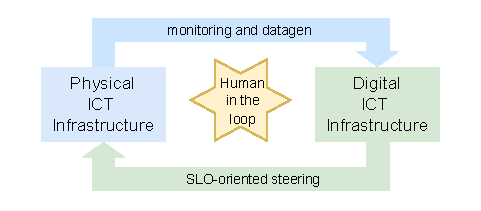
\includegraphics[width=0.98\linewidth]{report/figures/high-level-overview-dt-pt.pdf}
    \vspace*{-0.2cm}
    \caption{High-level overview of datacenter digital twinning system. The Physical ICT infrastructure collects telemetry data and directs it to the Digital ICT infrastructure, which, through simulation, offers back adjustment feedback best-aligned with the active SLOs. A human in the loop oversees the process and ensures the correctness and ethicality of the process. Adapted with permission from~\cite{Iosup2024DigitalTwins}.}
    \label{fig:high-level-element}

    \vspace*{-0.7cm}
\end{figure}

% \begin{itemize}
%     \item A data-driven digital shadow of a SURF datacenter that replays real workloads, visualizes power \& CO$_2$, and proposes simulation-based mitigations when issues arise.
%     \item Datacenter-level view (scheduler $\rightarrow$ nodes $\rightarrow$ jobs), representing how tasks are placed and executed across CPU/GPU nodes.
%     \item Public SURF traces (jobs + node telemetry) with timestamps enabling time-aligned replay; dataset available on Zenodo.
%     \item Simulation for decision support, ``what-if'' scenarios for failures, overloads, or carbon-aware scheduling (e.g., rescheduling a hot rack, delaying non-urgent jobs to lower-CO$_2$ windows, or shifting CPU/GPU placement) \textcolor{red}{TBD}
%     \item Understand how the real datacenter manages tasks over time, reduce energy/CO$_2$, and improve resilience
%     \item Use ML to forecast near-term load/power and CO$_2$, detect anomalies or impending failures, or recommend carbon-aware scheduling actions that cut energy and improve resilience. \textcolor{red}{TBD}
% \end{itemize}

Digital twinning ICT infrastructure is a novelty in computer systems and is innovative beyond the science of computer systems. However, in large-scale sciences such as aviation and space exploration, digital twins have been successfully used for decades, providing course-grained and dynamic adjustment the physical twin (e.g., airplanes, spaceships), from a distance, without physical access to the physical twin, yet only with operational access to the physical twin for dynamic adjustments aided by simulators coupled with live telemetry~\citationsneeded{3}. In small-scale sciences, such as applied biomedicine in cardiovascular health, digital twinning (eco)systems use patient-specific live telemetry (e.g., fusing imaging (e.g., MRI, CT), biosignals (e.g., ECG, electrocardiographic imaging)), and detailed physics-based electrophysiology simulation to predict treatment. ~\cite{sel2024building}. In contrast, to adopt a digital twinning operational ecosystem for complex datacenter ecosystems, medium-scale telemetry and models must combine higher-level abstraction with detailed monitoring and operational models for specific devices, applications, while addressing various operational phenomena~\cite{nicolae5377101m3sa}. This is fundamentally different from other-scale sciences~\cite{allen2019hierarchy, nicolae5377101m3sa}.

In this work, we address the open challenge of \textit{monitoring and operating massive-scale computer ecosystems through digital twinning}, by designing OpenDT, a first-of-its-kind ecosystem for datacenter digital twinning, implementing a prototype of the scientific instrument, and evaluating with realistic, trace-based experimentation scenarios. Adhering to the community-vetted, state-of-the-art AtLarge vision on researching distributed systems and ecosystems~\cite{iosup2019atlarge}, this paper contains a three-fold contribution:


% \todoall{There is currently no reference architecture of a digital twin. This is an issue: an ecosystem for distributed computer ecosystems can only be rigorously designed if it can be mapped to an existent, preferably also peer-reviewed, reference architecture... We can also play "the scientist" game, but this design otherwise is not robust science...}

\begin{enumerate}[label=\textbf{C\arabic*}]
\item \label{introduction:c1} (\textbf{Design}) We design OpenDT (steps 1-4 from \cite{iosup2019atlarge}, the first \underline{open}-source operational ecosystem for \underline{d}igital \underline{t}winning datacenters (\Cref{sec:design}). We formulate functional and non-functional requirements, then analyze design choices of OpenDT against the established requirements. We further the design of OpenDT and propose an operational workflow for the digital twinning ecosystem. We design the simulator component as generic, integrable with discrete-event simulators. Overall, OpenDT is modular and allows for each component to have various internal designs and implementations.

\item \label{introduction:c2} (\textbf{Prototype and experimentation}) 
We prototype OpenDT in \Cref{sec:prototype} (step 5 from \cite{iosup2019atlarge}). For the simulation component, OpenDT integrates OpenDC~\cite{DBLP:conf/ccgrid/MastenbroekAJLB21}, a peer-reviewed, state-of-the-art datacenter simulator, with over 8 years of operational experience and employed in national-scale projects (e.g., 6G Future Network Services~\cite{FutureNetworkServices2025}) and European-scale projects (e.g., Graph Massivizer~\cite{GraphMassivizer2025}). Then, in \Cref{sec:experiments}, we conduct three experiments (step 6 and 7~\cite{iosup2019atlarge}) aided by OpenDT to: (i) exp 1 (maybe show a real-world scenario and how digital twinning be better than just simulation), (ii) exp 2 (tbd), (iii) exp 3 (tbd). Overall, OpenDT enables ... 
\todoall{add findings here}.

\item \label{introduction:c3} (\textbf{Open Science}) 
 yWe contribute to open science all the software and data used and created in this project. We engineer OpenDT in (todo add the language), coupled with OpenDC, and with a demonstrational telemetry and feedback system, all supervised by a human-in-the-loop. For the experimentation phase, we use real-world traces collected from SURF~\footnote{\url{https://www.surf.nl}}, the largest datacenter provider in the Netherlands, align with OpenDT and OpenDT input requirements, and release the resulting input and output set as a FAIR dataset. Last, make available the complete reproducibility capsule: \todoall{actually make this capsule and add the link here.}


\end{enumerate}
 




\section{Background: Simulations, Shadows, Twins}\label{sec:background}

\begin{figure}
    \centering
    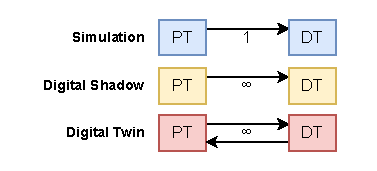
\includegraphics[width=0.75\linewidth]{report/figures/background.pdf}
    \caption{High-level overview and comparison of physical twin (PT) and digital twin (DT) interaction in simulation, digital shadowing, and digital twinning.}
    \label{fig:background}
\end{figure}

In this section, we present background on datacenter simulation, digital shadowing, and digital twinning, and a high-level comparison between these operational techniques illustrated by \Cref{fig:background}.

\begin{figure*}[h]
    \centering
    \hspace*{-0.55cm}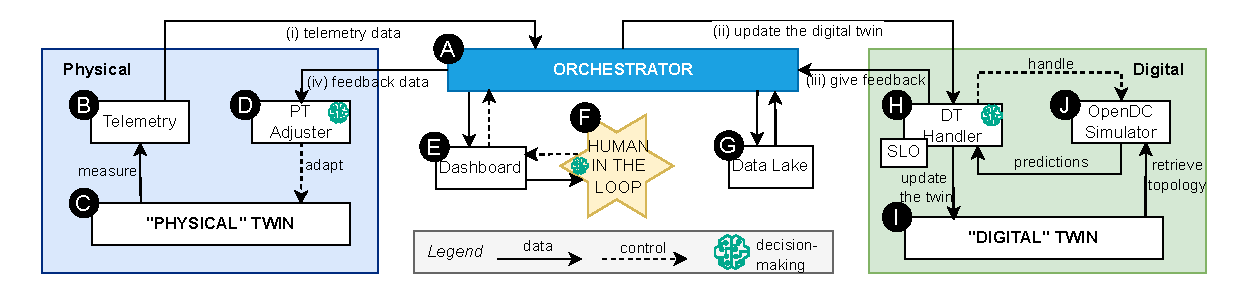
\includegraphics[width=1.05\linewidth]{report/figures/opendt-design.pdf} 
    \caption{Architecture overview of OpenDT, a digital twinning ecosystem for monitoring and operating datacenters.}
    \label{fig:opendt-design}
\end{figure*}

\textit{``Simulation is defined as the imitation of the operation of a system or real-world process over time, and in many cases, manufacturing provides one of the most important application of simulation"}~\cite{DBLP:conf/wsc/LeeMS03, nicolae5377101m3sa}. Simulation provide datacenter stakeholders with operational insights on infrastructure under workload~\cite{nicolae5377101m3sa}. The top third of~\Cref{fig:background} illustrates simulation as a unique-state prediction task of the physical twin under a simulation scenario. Simulators use \textit{predictive models}, empirical prediction systems that analyze, combine, and compute various input elements to produce fine-grained output predictions~\cite{modsim:book/ZaraiN15:orig, nicolae5377101m3sa}.

\textit{``A Digital Shadow is a set of temporal data traces and/or their aggregation and abstraction collected concerning a system for a specific purpose with respect to the original system.}~\cite{Braun2023_DigitalShadowDefinition}. The middle third of~\Cref{fig:background} illustrates a digital shadowing system which, unlike the single-event of simulation, the digital twin component continously mirrors the physical twin and optionally tracks the state of the physical twin over time.


\textit{``A digital twin is an integrated data-driven virtual representation of real-world entities and processes, with synchronized interaction at a specified frequency and fidelity."}~\cite{DTC_Digital_Twin_Definition_2025}. The bottom third show of~\Cref{fig:background} illustrates the continuous interaction loop between the physical twin, which communicates telemetry data to the digital twin; the digital twin, aided by simulation, suggests SLO-oriented adjustments to the physical twin.

Simulation enables fine-grained datacenter operational monitoring used by stakeholders in decision-making processes~\cite{nicolae5377101m3sa}. \textit{Workloads} contain tasks operated on \textit{infrastructure}, which includes physical machines, virtual machines (VMs), and containers~\cite{nicolae5377101m3sa}. Traces represent recordings or real-world events capturing detailed operational data of the infrastructure under given workload(s)~\cite{nicolae5377101m3sa}.
% Further
% Paragraph on terminology (workload, traces, etc)

% \begin{figure}[t]
%     \centering
%     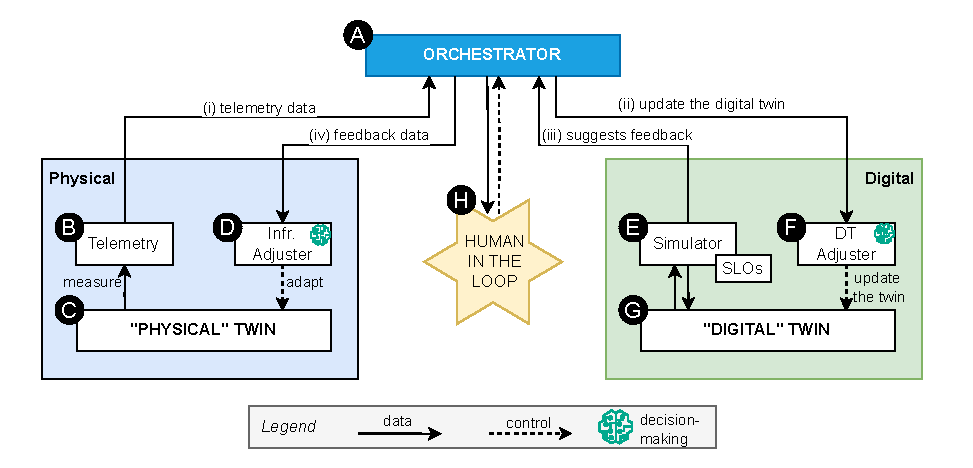
\includegraphics[width=\linewidth]{report/figures/DT-reference-architecture.pdf}
%     \caption{Caption}
%     \label{fig:placeholder}
% \end{figure}


% ======================================
% IMPORTANT - DO NOT DELETE
% IMPORTANT - DO NOT DELETE
% IMPORTANT - DO NOT DELETE


% \subsection{Reference Architectures}

% \subsubsection{Cardiology}

% Recent surveys converge on a layered architecture for digital cardiovascular twins. Data acquisition and integration fuse multimodal streams (wearables and home sensors, ECG/PPG, cardiac imaging, laboratory tests, and EHR), providing a continuously synchronized patient state. In addition to this, domain models combine multiscale cardiac physiology (electrophysiology and hemodynamics) with data assimilation to personalize parameters and quantify uncertainty, while learned surrogates accelerate interfence for clinical workflows based on time. The analytics and decision support then deliver the prognosis, the optimization of therapy and the 'digital trial' of scenarios through clinical interfaces governed by validation, traceability and privacy policies \cite{sel2024building}\citationsneeded{2}.

% \todoall{COMPARE RA \cite{sel2024building} to OPENDT fig or table}

% \subsubsection{Water Systems}

% For water distribution, reference designs resolve around a cyberphysical loop: telemetry via SCADA (pressures, flows, pump/valve states) and network metadata feed a hydraulics backbone augmented with learning-based estimators for partially observed systems; anomaly and change detection trigger model evolution; and operator dashboards translate insights into pump scheduling, valve manipulation, and maintenance priorities \cite{DBLP:conf/isola/DegelerYKLLTT24}\citationsneeded{2}.

% \todoall{COMPARE RA \cite{DBLP:conf/isola/DegelerYKLLTT24}  to OPENDT fig or table}


\section{Design} \label{sec:design} 

% In this section, we synthesize requirements and design the architectures of two models of different architectural complexities.

In this section, we synthesize requirements and design two models of opposite architectural complexities.



\begin{figure*}
    \centering
    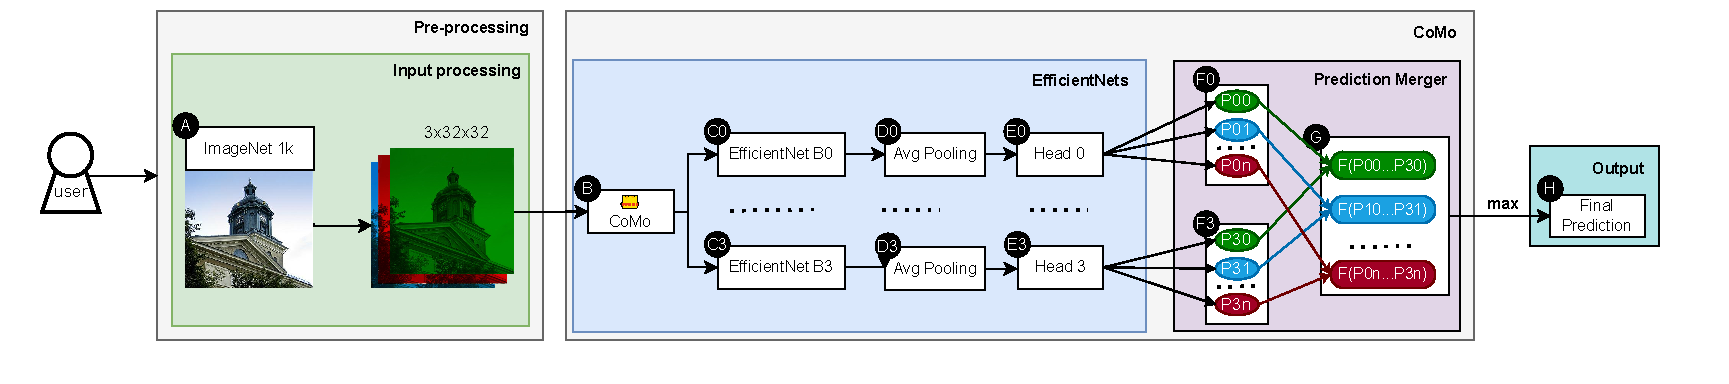
\includegraphics[width=0.95\linewidth]{figures/design-como.pdf}
    \caption{A high-level architectural overview of CoMo, a complex architectural model.}
    \label{fig:design:como}
\end{figure*}

\subsection{Requirement Analysis} \label{sec:m3sa:requirements-analysis}
%\begin{enumerate}[label=\textbf{(FR\arabic*)}, leftmargin=3em]
\begin{enumerate}[label=\textbf{(FR\arabic*)}, leftmargin=0pt, itemindent=3em]
    \item \label{fr1} \textbf{\underline{Si}mple architectural \underline{Mo}del for object classification} This research should involve a simple architectural model, the SiMo model. Despite the inherent simplicity, SiMo should be able to conduct object classification, while still meeting the other functional and non-functional requirements.
    
    \item \label{fr2} \textbf{\underline{Co}mplex architectural \underline{Mo}del for object classification}: 
    This research should involve a complex architectural model, CoMo, able to conduct object classification. CoMo should predict using under the hood multiple open-source, peer-reviewed, and community-vetted models, and integrate their predictions into a final prediction, thus filtering individual model biases, and enhancing prediction reliability.    

    \item \label{fr3} \textbf{Open-source and reproducible}: 
    Data created and used in this work should be open-sourced, following the principles of open science. Experiments should be reproducible.
\end{enumerate}

\begin{enumerate}[label=\textbf{(NFR\arabic*)}, leftmargin=0pt, itemindent=3em]
    \item \label{nfr1} \textbf{Provide live, instantaneous predictions}: 
    Both SiMo and CoMo should be able to classify first-time-seen, individual objects under 2 seconds. The models should be able to each predict batches of 100 images under 1 minute.
    
    \item \label{nfr2} \textbf{Highly accurate predictions}: 
    Models' accuracy should be at least 8 times higher than the guessing factor (e.g., for 16 classes the guessing factor is $6.25\%$; models'  accuracy should be at least $ 8\cdot6.25\%$).
    
    \item \label{nfr3} \textbf{Leverage four, peer-reviewed, community-vetted models}: 
    CoMo should employ four peer-reviewed and community-vetted individual models, and leverage their predictions into an atomic prediction.

    \item \label{nfr4} \textbf{Multiple-class operability}: 
    CoMo and SiMo should predict at least 16 classes of objects. This limited and computer science round number, should serve as a proof of concept, and suffice the research and experimental basis of this work.

    \item \label{nfr5} \textbf{Limited resources operability}: 
    Training and inference should be conducted on a small-sized cluster (i.e., not a supercomputer), while still meeting all the aforementioned requirements.

    
\end{enumerate}


\subsection{Design of SiMo, a \underline{Si}mple architectural \underline{Mo}del}\label{sec:design:simo}

SiMo (Simple architectural Model) architecture is designed to provide a straightforward yet effective solution for object classification tasks. The term ``simple" refers to SiMo's relative simplicity in comparison to more complex models while still being sufficiently sophisticated to meet the functional and non-functional requirements\ref{fr1}. For this purpose, SiMo employs a 3-layer convolutional neural network (CNN), providing a balance between depth and efficiency and ensuring that the model captures complex patterns without excessive computational costs.

We train, validate and test SiMo on Imagenet-1k \cite{DBLP:conf/cvpr/DengDSLL009}, a large scale dataset commonly used for benchmarking and consisting of 1000 classes, thus ensuring SiMo fulfills \ref{nfr4}.

Figure \ref{fig:design:f3} depicts a high-level overview of SiMo. The process of SiMo begins in step \circled{A}. After data pre-processing (further expanded in \Cref{sec:implementation}), the input image is fed into the network. The network itself consists of three convolutional layers (\circled{B1}-\circled{B3}), each progressively increasing the number of output nodes (\circled{B1} contains 64 output nodes, \circled{B2} contains 128 output nodes, \circled{B3} contains 256 output nodes). This simple yet powerful design choice allows the network to capture a wide range of features, from simple patterns in early layers to more complex representations in the deeper ones \ref{nfr2}. We apply batch normalization after each convolution to stabilize training and keep values in the network within a reasonable range \cite{NEURIPS2018_905056c1}. We use ReLU activation to introduce non-linearity as it is a standard practice in neural networks \cite{rasamoelina2020review}. 

Furthermore, this design utilizes 5x5 MaxPooling after each convolutional layer to reduce the spatial dimensions of the feature maps, increasing the model's efficiency by reducing complexity while still preserving the main information needed for accurate predictions.

Unlike deeper architectures, SiMo does not include dropout, as its shallow design inherently limits overfitting. Overfitting is a concern in deeper networks with millions of parameters, but SiMo’s simplicity naturally mitigates this risk. Adding dropout would introduce unnecessary stochastic operations, slowing down both training and inference \ref{nfr1} without providing meaningful gains in accuracy or generalization \ref{nfr2}.

Lastly, after passing through the convolutional layers, the output is flattened and passed to a fully connected layer \circled{C} with 1000 output units, corresponding to the number of classes and ensuring \ref{nfr4} is met, which performs the classification in step~\circled{D}. This final layer ensures that SiMo remains lightweight and efficient \ref{nfr1}. 

This overall design choice, with the high-level picture depicted in \Cref{fig:design:simo}, allows SiMo to strike a robust balance between simplicity and performance, making the model well-suited for object classification tasks where computational resources are limited. In \Cref{sec:experiments}, we analyze the performance of SiMo prototype embodying the architecture depicted in \Cref{fig:design:simo}, and able to predict 1,000 classes. We measure an accuracy of 34.37\%, and the ability to run on average 5795.5 samples per second.



% ==================================================================================================================



\subsection{Design of CoMo, a \underline{Co}mplex architectural \underline{Mo}del}\label{sec:design:como}

CoMo, a Complex Architectural Model, is designed for highly accurate object detection despite posing an inherent complexity \ref{fr2}. \Cref{fig:design:como} depicts an overview of CoMo architecture, in which CoMo embeds four versions of EfficientNet \cite{tan_efficientnet_2020}, a vetted, state-of-the-art, and widely used family of models, with proven accuracy and performance on datasets as CIFAR-100 or Flower~\cite{DBLP:conf/icml/TanL19}. We train, validate, and test the CoMo using ImageNet-1k\cite{DBLP:conf/cvpr/DengDSLL009}, a large-scale dataset, with 1,000 classes, thus ensuring the multiple-class operability of CoMo \ref{nfr4}.

We design CoMo as able to integrate versions B0, B1, B2, and B3 of the EfficinetNet family \ref{nfr3}, yet design and engineer CoMo as simply expandable to higher iterations of the EfficientNet. This design serves as a proof of concept that is especially relevant for testing out prototypes of financially costly machine learning applications. We archive our design goals by building CoMo under limited computation resource availiable; we argue that, albeit valuable for CoMo to include up to iteration B8, such a design would result in an unfeasible model for the limitations of this research. We thus regard B0-B4 as sufficient to meet complexity requirements \ref{fr2}, model multiplicity \ref{nfr3}, and accuracy requirements \ref{nfr2} while still meeting the requirement of limited resources operability \ref{nfr5}.

\textit{Input processing step:} The CoMo process begins in step~\circled{A}, with an image provided by the user, e.g., an image from the test split of ImageNet-1k. The image undergoes pre-processing and resides in a three-dimensional tensor of size 3x32x32, thus ensuring uniformity across inputs and compatibility with the EfficientNet models. The processed input is then fed into CoMo (\circled{B}).

\textit{EfficientNets step:} CoMo underlies four versions of EfficientNet, run in parallel, and each sub-model predicts without interfering with one another~\ref{fr2}. Besides, each submodel underlies an identical architecture and has a single differing element, the version of the EfficientNet (\circled{C0} - \circled{C3}); thus, to prevent redundancy, we will further detail only the submodel using EfficientNet B0. The predictions B0 are fed into an average pooling layer (\circled{D0}), which compresses the spatial information into a fixed-length vector by averaging the values in each feature to produce a single value per channel. Further, the input is fed into a head (\circled{E0}), which flattens the pooling layer and classifies the image, thus preparing predictions for the aggregation step.

\textit{Prediction aggregation step:} The prediction merger component is designed to maximize accuracy \ref{nfr2} by alleviating individual model biases and filtering out extremes, thus strengthening prediction robustness. In elements~\circled{F0} - \circled{F3}, the system leverages predictions of each submodel per each class. \Cref{fig:design:como} labels the predictions following the structure P[model id][class id] (e.g., P01 represents class 1 of model 0). The leveraged predictions are further fed into an aggregation function, which combines the predictions (\circled{G}). After applying the aggregation function, the class with the highest probability is selected as the final prediction and delivered as the output of the system (\circled{H}).

Choosing an aggregation function for element \circled{G} is a non-trivial process that needs to address the accuracy complexity trade-off.
The function used in \circled{G} could be either a statistical function (e.g., mean, median) or ML-based. We further analyze the benefits of each approach. Firstly, statistical functions could be a computational light approach, with (arithmetic) \textit{mean} used for aggregating predictions in datacenter simulation~\cite{nicolae2025m3sa}, ecology~\cite{harrison2018brief}, and meteorology~\cite{myhre2017multi}, but has a high sensitivity to outliers, and \textit{median}, which alleviates the outlier sensitivity of the mean but is more computationally expensive~\cite{nicolae2025m3sa}. Secondly, ML-based aggregation functions would add extra complexity and computation time, which would hinder and bias the performance and accuracy comparison between the core architectures of SiMo, a model comprising only three hidden layers, and CoMo, a model embodying four large-scale pre-trained models; an additional heavy-weight computation in the aggregation component could improve the overall accuracy \ref{nfr2}, but bias the measurements from \Cref{sec:experiments}, thus deviating from the original purpose of \ref{introduction:mrq}. We, therefore, choose the statistical approach and combine predictions using (arithmetic) mean.  

These design choices, synthesized into the high-level architecture from \Cref{fig:design:como}, allow CoMo to balance complexity with performance and accuracy. In \Cref{sec:experiments}, we analyze the performance of a CoMo prototype embodying the architecture described in this section and are able to predict for 1,000 classes; we further compare CoMo with SiMo on various metrics. We quantify CoMo and obtain an accuracy of 57.8\% and the ability to run on average 321.63 samples per second. The measured throughput (samples/sec) for mile-predictions of SiMo is 18 times bigger than that of CoMo.

\section{Implementation of an OpenDT prototype}\label{sec:prototype}
In this section, we present implementation details of OpenDT, matching step 5 from the community-standard research methodology on the distributed systems. In this early prototype, due to time resource constrains, we couple OpenDT with data obtained from a real-world datacenter and used in peer-reviewed literature; we planned future work in coupling OpenDT with real-world ICT infrastructure, which would send telemetry data to the OpenDT and receive adjustment feedback from OpenDT.


\subsection{Dataset}\label{sec:dataset}

To replicate the real-world infrastructure (i.e., physical twin), we replay data from the FAIR dataset of SURF-22, a scientific workload trace used in peer-reviewed experiments~\cite{DBLP:conf/wosp/NiewenhuisTIM24, nicolae5377101m3sa}. SURF-22 was traced in one of the largest HPC facilities at SURF, Netherlands, over 7 days, in October 2022, and contains anonymised scientific jobs run in production, batch, with an average duration of 39.52 CPU-hours and also detailed energy use over the same period~\cite{nicolae5377101m3sa}. The SURF workload contains 7,850 tasks, and 2,323,475 corresponding fragments, spanning in total approximately 310,000 CPU hours, and are sampled at a granularity of 30 seconds~\cite{nicolae5377101m3sa}. Many thanks to AtLarge Research and our collaborators from SURF for the FAIR dataset released to open-science.


\begin{table}[t]
\centering
\renewcommand{\arraystretch}{1.1}
\begin{tabularx}{\linewidth}{l l l X}
\toprule
\textbf{Field} & \textbf{Data type} & \textbf{Unit} & \textbf{Description} \\
\midrule
id               & string   & —    & Unique identifier \\
duration         & int64    & ms   & Duration of task \\
submission\_time  & datetime & —    & Time of task submission \\
cpu\_count       & int32    & count& Number of CPUs required \\
cpu\_capacity     & float64  & MHz  & CPU capacity required \\
mem\_capacity     & int64    & MB   & Memory required \\
\bottomrule
\end{tabularx}
\caption{Schema of the tasks dataset. A workload task compatible with OpenDC contains multiple fragments, as detailed in~\cite{opendc-workload}.}
\label{tab:tasks_schema}
\end{table}


\begin{table}[t]
\centering
\renewcommand{\arraystretch}{1.1}
\begin{tabularx}{\linewidth}{l l l X}
\toprule
\textbf{Field} & \textbf{Data type} & \textbf{Unit} & \textbf{Description} \\
\midrule
id            & string  & —    & Unique identifier \\
duration      & int64   & ms   & Duration of fragment \\
cpu\_count     & int32   & count& Number CPUs used in fragment \\
cpu\_capacity  & float64 & MHz  & CPU capacity used in fragment \\
\bottomrule
\end{tabularx}
\caption{Schema of the fragments dataset. OpenDC is compatible with the fragments schema explained in~\cite{opendc-workload}.}
\label{tab:fragments_schema}
\end{table}

\Cref{tab:tasks_schema} presents the schema underlying the tasks component and \Cref{tab:fragments_schema} presents the schema of the fragments component of the SURF-22 dataset. In the SURF-22 workload, OpenDC-compatible, fragments are ordered and grouped into chunks and all the fragments beloning to a task share the same id, specifically the ID of the parent task.

\textit{Performed data processing:} The FAIR dataset of SURF-22 was already compatible with OpenDC, thus we did not conduct any data processing steps. However, in the past, the SURF-22 dataset has been processed by AtLarge Research Group mainly by anonymizing the scientific tasks, ensuring exact compatibility between the data file received from SURF and the input schema needed by OpenDC, and, ultimately, releasing the resulting data file as a FAIR dataset.

We use the SURF-22 dataset as a temporary replacement for the physical twin component. We have planned future work in coupling OpenDT with physical twin, which would provide real-time, real-world telemetry to the digital twinning ecosystem OpenDT underlies. In a real-world setup, similarly, OpenDT would receive telemetry data of both the workload (e.g., which tasks need to be executed, estimated time) and sensor-measured telemetry data (e.g., hardware resource utilization, energy consumption, temperature, cooling).


\subsection{Processing windows} \label{sec:processing_windows}
OpenDT contains a (virtual-) physical twin, underlying Apache Kafka, a state-of-the-art distributed event log and streaming platform, widely used in the community for high-throughput event streaming, and durable event history storage~\cite{kafka, kreps2011kafka}. We configure a replaying granularity of 5 minutes, following the industry standard~\cite{DBLP:conf/ccgrid/MastenbroekAJLB21, DBLP:journals/fgcs/MastenbroekMBI25}, based on the timestamp of the task, and, thus, of the fragment. The starting time of the replay is the smallest timestamp from the workload trace. After every window, the state of the digital twin is multi-layer updated: the simulation component predicts energy consumption and resrouce utilization, the newly arrived tasks are considered, the LLM's suggestions of topology improvement are displayed, awaiting for user's acceptance, etc. 

For demonstrational purposes, we implement a configurable ratio between the replay granularity and the demo-granularity; for example, if the real-world granularity is 300 seconds (i.e., 5 minutes), Kafka streams from SURF-22 pre-defined file, and the ratio is 1:10, the 5 minutes of (virtual-)real-world operation would be executed within 30 seconds. A granularity of 1:100 and 300 seconds of (virtual-)real-world operation would lead to 3 seconds. 

\subsection{Operations done in a processing window}
All the algorithms and analyses are conducted at the window granularity and, thus, an identical process is performed for each window. 
Firstly, OpenDC simulator predicts, for each window, the SLO objectives (e.g., predicts the energy consumption and execution time of the workload in subject). 
Secondly, the OpenDT orchestrator processed the OpenDC's predictions and forwards them to an LLM component (further expanded in~\Cref{sec:design:llm}), which assesses the alignment with the practitioner-established SLOs and, if needed, suggests the practitioner topology adjustments towards fulfilling the SLOs. 
Thirdly, the LLM outputs topology adjustments and displays them to the dashboard, where the human-in-the-loop can approve or reject the changes (we expand the crucial importance of the human-in-the-loop for major decisions in~\Cref{sec:design:choices}).
Lastly, on the approval of the supervising practitioner, the infrastructure is adjusted. 
All data is saved in a datalake, thus aiding for potential investigation, operation, or processing such as historical replay, operational analysis, or incident reports. 



\subsection{Visualization and System Outputs}

The OpenDT platform prototype has a unique control panel that shows the current state of the system, including the datacenter topology and information about current tasks and fragments. The main view \Cref{fig:dashboard} focuses on the details of the current simulation powered by the Digital Twin. This allows operators to analyze the information and take decisions from a single interface, instead of using multiple tools.

\begin{figure}[t]
    \centering
    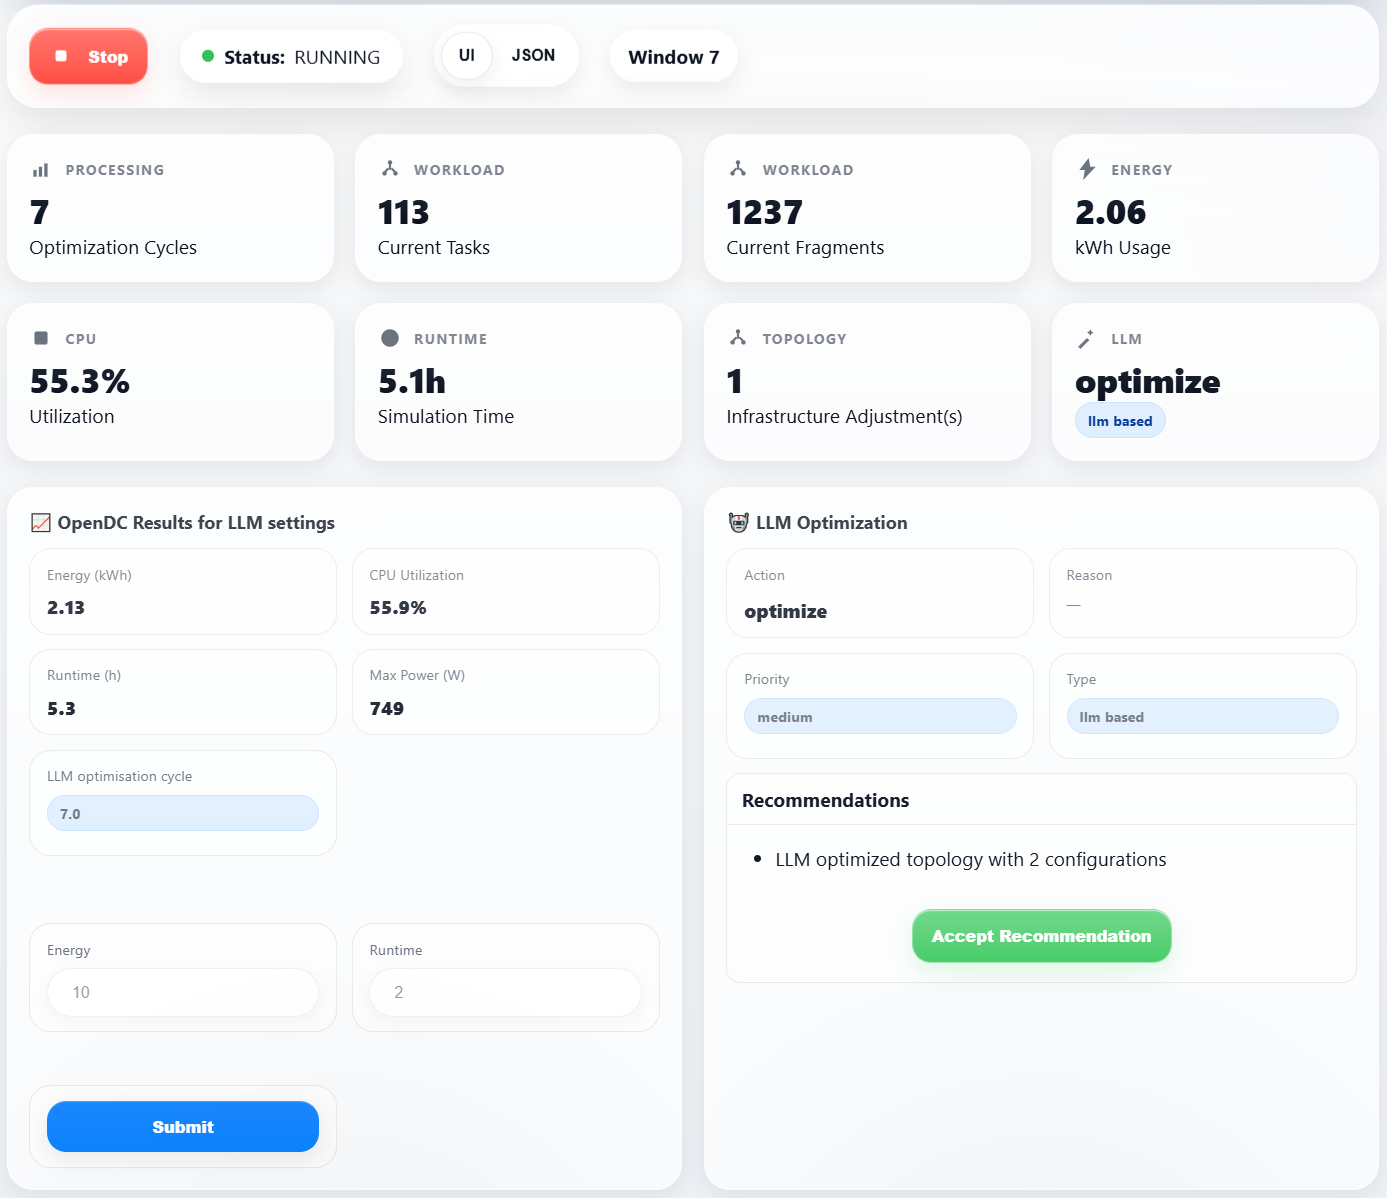
\includegraphics[width=\linewidth]{figures/dashboard.png}
    \caption{OpenDT Digital Twin Dashboard integrating real-time telemetry, simulation results, and LLM-guided topology recommendations.}
    \label{fig:dashboard}
\end{figure}

The panel shows the following useful data: optimization cycles, workload (current task and fragments), energy usage (kWh), CPU utilization, simulation time, and current topology. In addition, an optimization panel can be found. The panel allows the operator to set the energy and runtime in alignment with the SLO's that are then feed into the LLM model for the optimization process.  Afterwards, the operator can accept the recommended topology. The recommendations appear in the same panel, or it can be viewed as a structured JSON record.

Additionally, the visualization has three real-time plots that allow for a direct comparison between the physical and digital twins. \Cref{fig:cpu_plot} shows the evolution of CPU utilization over time. The blue line is the telemetry data obtained from the real datacenter, while the orange dashed line is the result from the OpenDC simulation. The alignment of the two curves can indicate a correct mapping of the workload and allows the operator to identify general use patterns.

\begin{figure}[t]
    \centering
    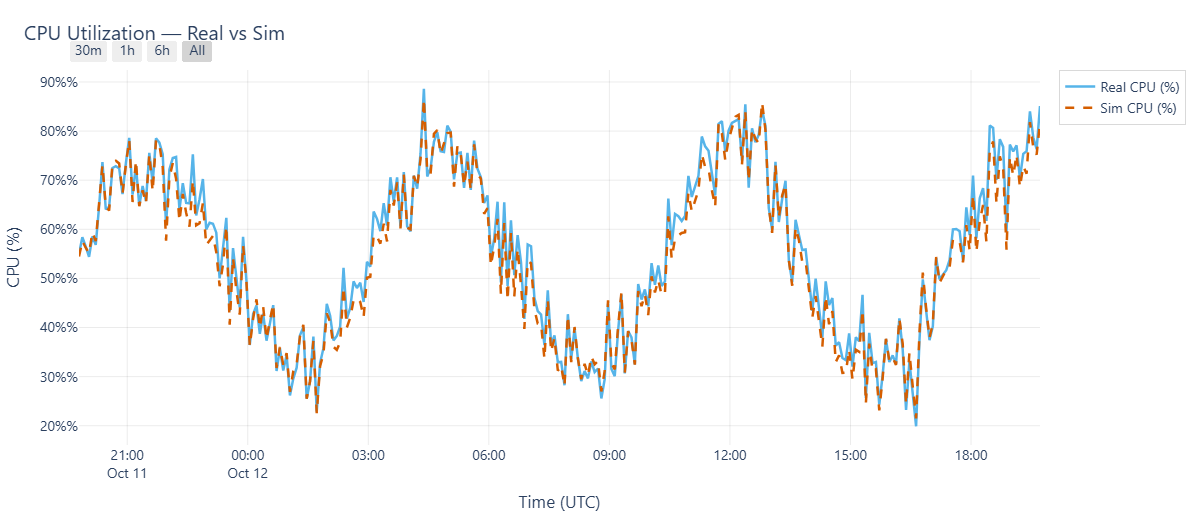
\includegraphics[width=\linewidth]{figures/cpu_plot.png}
    \caption{CPU utilization comparison between real and simulated datacenter telemetry.}
    \label{fig:cpu_plot}
\end{figure}

Similarly, \Cref{fig:power_plot} shows the energy consumption (watts). The main objective of this view is to outline the energetic behavior between twins in the short term. If the lines diverge during a specific window it can be due to heavier or workloads or fails in the hardware of the physical twin (such as cooling problems) that are not yet implemented. Even so, the operator can use this to quickly alert or take action if needed.

\begin{figure}[t]
    \centering
    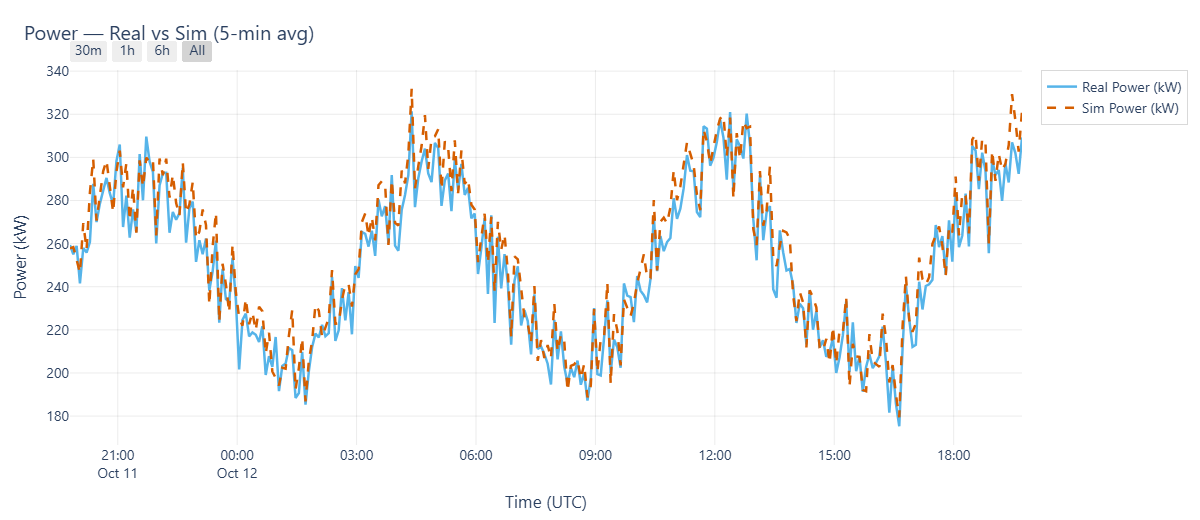
\includegraphics[width=\linewidth]{figures/power_plot.png}
    \caption{Power draw comparison between real and simulated telemetry.}
    \label{fig:power_plot}
\end{figure}

Lastly, ~\Cref{fig:energy_plot} shows the cumulative energy consumption (in kWh) calculated from the power traces. This offers a different point of view focused on the long-term of simulations. A close match between both curves indicates that OpenDT maintains accurate energy estimation across simulations.

\begin{figure}[h]
    \centering
    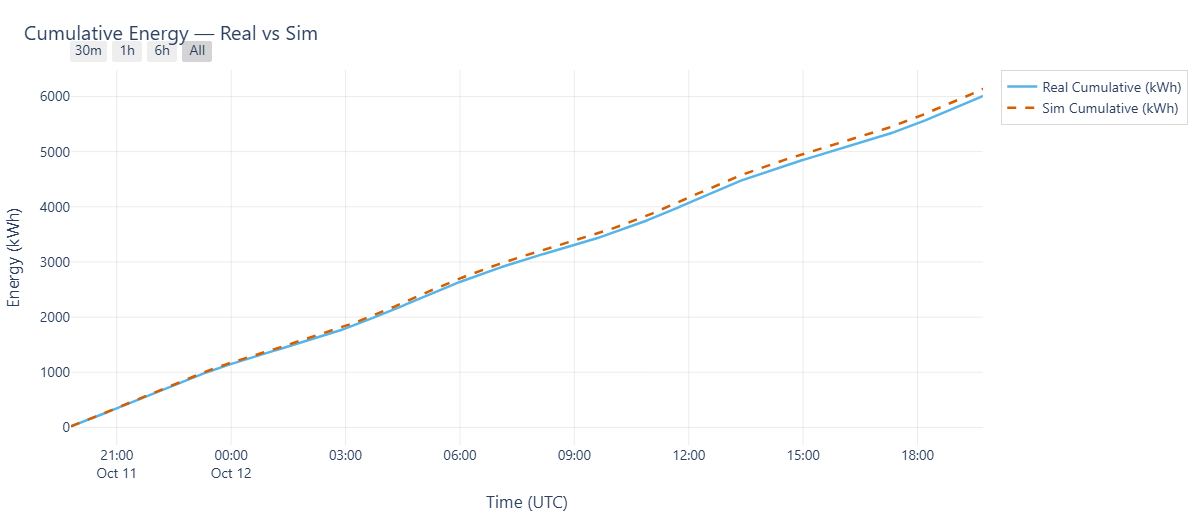
\includegraphics[width=\linewidth]{figures/energy_plot.png}
    \caption{Cumulative energy consumption comparison between physical and digital twins.}
    \label{fig:energy_plot}
\end{figure}

In general, the OpenDT interface transforms the digital twin from a passive simulator into a real-time decision-making tool. By integrating real telemetry and simulation data, with topology recommendations align with clear objectives, allows operators to analyze and verify the fidelity of the digital twin. Furthermore, detecting anomalies and aligning the capacity of the datacenter with SLO's becomes easier and more direct by allowing multiple simulations in a short amount of time. In other words, visualization not only communicates data, but also provides continue feedback between the system and the humans in the loop, making the process interpretable, trustworthy, and actionable in real-world datacenter operation.
\section{Reflection}\label{sec:reflection}

In this section, we reflect on the performed work, discuss challenges and opportunities arising from this work, and discuss potential future improvements and research deriving from the OpenDT prototype. 

\subsection{Use cases and requirement assessment}\label{sec:reflection:use-case-requirements}
In this section, we reflect on how our work addresses the use-cases and requirements identified in \Cref{sec:design}.

\begin{enumerate}
[label=\textbf{(UC\arabic*)},leftmargin=0pt,itemindent=3em]
    \item \label{design:uc1} \textbf{Monitoring and operation datacenters}: The current design allows datacenter operators to both monitor and operate massive-scale datacenters. The implemented prototype, functioning as a digital shadow, allows operators to monitor datacenter behaviour, assuming correct linking with a telemetry component, fed with real-world data, with an existing physical twin, and allows operators to conduct what-if analysis in a time and cost efficient way.
    \item \label{design:uc2} \textbf{Researching ICT Infrastructure} The current design and prototype enable stakeholders from the scientific community to experiment with digital twinning ICT infrastructure by building and functional a prototype, also the first and unique digital twinning ecosystem for monitoring and operating ICT infrastructure, aided by LLMs. Our scientific instrument can benefit the scientific community by analyzing how different datacenter configurations would behave under different configurations and under various operational phenomena. Futhermore, OpenDT enables researchers to evaluate the role and abilities of LLMs in operating and SLO-aware adjusting ICT infrastructure.
    \item \label{design:uc3} \textbf{Education} OpenDT can aid students to conduct real-time and continuous what-if analysis on ICT infrastructure under various configurations and running various workload traces. Furthermore, OpenDT can aid as a lab tool in computer systems and digital twinning courses, such as Computer Organization or Distributed Systems, or MOOC courses on edX.
\end{enumerate}

\subsection{Requirement Analysis}\label{sec:design:requirements}
We now assess OpenDT's alignment with the established requirements. We first evaluate whether OpenDT meets the functional requirements.

\begin{enumerate}[label=\textbf{(FR\arabic*)},leftmargin=0pt,itemindent=3em]
    \item \label{design:fr1} \textbf{Digital twin physical ICT infrastructure}: 
    OpenDT receives continuous input from a data broker handled by Apache Kafka, simulates the environment, displays results on a dashboard in real time, thus mimicking a potential real-world ICT infrastructure, and suggests LLM-provided feedback for adjustments such that the datacenter is aligned with SLOs. Albeit essential for a digital twinning ecosystem, the current prototype is not (yet) coupled with a real-world physical datacenter due to the infrastructure and time limitations.
    \item \label{design:fr2} \textbf{Simulate with state-of-the-art scientific instrument}: 
    OpenDT uses OpenDC as a representation model of the system and environment. OpenDC is a peer-reviewed, discrete-event datacenter simulator, community and industry-vetted, widely used in scientific venues and National/European scale projects. Thus, we regard OpenDC as a reliable and most suitable ICT simulator, and couple it with OpenDT as the simulation component, specifically component \circled{J} from~\Cref{fig:opendt-design}.
    \item \label{design:fr3} \textbf{Suggest SLO-aligned changes of the physical twin}: 
    OpenDT suggests LLM-assisted topology adjustments such that the infrastructure under workload meets the practitioner-established SLOs. OpenDT allows the human-in-the-loop to select the topology best aligned with SLOs. The LLM component is present and implemented by the Digital Twin Handler, specifically component~\circled{H} from \Cref{fig:opendt-design}.
    \item \label{design:fr4} \textbf{Autonomous, human-in-the-loop validated}: 
    OpenDT is fully autonomous in monitoring the behavior of the physical twin. The design presented in~\Cref{sec:design} suggests fully autonomous adjustments of the infrastructure, LLM-based, when the adjustments are minor (e.g., reducing the computing power by 1\%), yet require a human-in-the-loop for major decisions (e.g., deciding the priority between two batches of tasks, both of very large-durations, and of various natures). The current prototype of OpenDT requires a human in the loop for approving LLM feedback and contains a flag for making the system fully autonomous; however, the current prototype lacks a decision-based process for distinguishing between minor and major decisions.
\end{enumerate}

We now evaluate OpenDT's adherence to non-functional requirements. However, we note that alignments to NFRs cannot be robustly conducted without robust testing and experimentation. However, according to the course rubrics, evaluation and validation of the performance and fidelity of the engineered prototypes is out of the scope of this report and, thus, skipped for this iteration of the OpenDT research.
\begin{enumerate}[label=\textbf{(NFR\arabic*)},leftmargin=0pt,itemindent=3em]
    \item \label{design:nfr1} \textbf{Rapid, efficient digital twinning}: 
    OpenDT is capable of simulating and receiving LLM feedback on infrastructure adjustments, all in a window 30 seconds between telemetry data. However, while these have been unstructuredly tested, also shown in the course's demo, a robust performance validation is yet to be conducted and envisioned as future work.
    
    \item \label{design:nfr2} \textbf{Accurate adjustment feedback}: 
    OpenDT prototype contains an LLM-based feedback adjustment component which uses the OpenAI's API for GPT 3.5 turbo. We thus conclude that the accuracy of the adjsutment feedback of the OpenDT's ecosystem is directly dependent on the accuracy of the implemented LLM and the structure of the LLM prompt.
    
    \item \label{design:nfr3} \textbf{Massive-scale operation}: 
    OpenDT's design supports massive-scale operation, as detailed in~\Cref{sec:design}. OpenDT's implemented prototype is engineered towards massive-scale operation; firstly, we use Apache Kafka for telemetry and data streaming, a messaging platform that is a state-of-the-art tool and recognized for its good-scalability properties and high throughput; secondly, the adopted simulator is peer-reviewed and community vetted for simulating large-scale workloads, highly accurate (with error rates of under 8\%) and rapidly (OpenDC can simulate months of operation within seconds).
\end{enumerate}



\subsection{Challenges}\label{sec:reflection:challenges}
Throughout the research and engineering process of OpenDT, we encountered various challenges, as expected especially when proposing a first of-its-kind-tool, aimed for massive-scale operation and adhering to industry standards. We divide these challenges in two main categories: challenges encountered during the design process and challenges encountered during the engineering process. Overall, following the methodology proposed and vetted in the community-standard methodology on designing, engineering, and researching distributed (eco)system, we conducted the design and engineering process iteratively and concurrently.

\textit{Design challenges and decisions:} Throughout the design process, we encountered three main challenges. 
1) The high-level design from~\Cref{fig:opendt-design} has been obtained after numerous iterations, on both the design and the engineering side. The main design challenge was determining the role of the machine learning model in predicting infrastructure improvements and the specific role of the human-in-the-loop. We expand on the design choices, considerations, and rationale in~\Cref{sec:design:choices}.
2) Once deciding the role of the machine learning algorithm, we evaluated the main candidates and chose between Reinforcement Learning and Large Language Model based suggestions for infrastructure improvement. After unstructured discussion with experts in computer systems, datacenter operation, and datacenter simulation, and based on these discussions, we concluded that infrastructure adjustment based on a Reinforcement Learning approach is already explored and over-explored, without major benefits to the community. In contrast, LLM is becoming the new state-of-the-art, is yet unexplored, and is becoming of increasingly more interest for the scientific community. We thus decided on implementing the machine learning component following  an LLM-based approach.
3) Cascading from the previous point, an LLM requires robust prompt engineering (although the name, this is still a design choice) to lead to reliable results. After consulting peer-reviewed literature in the field, and after iteratively testing, we adopted the prompt structure proposed in~\Cref{sec:design:llm}.

\textit{Engineering challenges} Similarly, on the engineering process we also encountered challenges, yet of a different nature.
1) Integrating Apache Kafka and ensuring compatibility with OpenDC has been a bottleneck for a few days. While the process itself is not difficult, the implementation, bug fixes, documentation analysis an re-analysis turned out to be more time demanding that initially expected. Yet, it was worth it! Kafka is state-of-the-art and highly scalable.
2) While each component functions well separately, integrating into an orchestrator (i.e., central authority), specifically component \circled{A} from \Cref{fig:opendt-design}, and making all the components tick at the same time, tick correctly, and tick in the correct order represented another main engineering challenge (however, we foresaw this one :D). 


\subsection{Future work}\label{sec:reflection:challenges}
We plan future work for OpenDT towards evolving the current digital twinning to an industry-standard digital twin, used in large-scale research projects and employed by datacenter practitioners in their monitoring and operational processes. Specifically, our plan is four-fold.

Firstly, we plan to link OpenDT with real-world datacenters, which would offer live and real-world telemetry and, in turn, OpenDT would give infrastructure adjustment suggestions, some autononmous, and some approved by a human-in-the-loop.

Then, secondly, we plan to evaluate the performance of OpenDT, the accuracy of OpenDT's LLM component, and how well various LLMs would perform, and, lastly, evaluate the ecosystem against extreme, yet real-world edge cases, evaluate for fault-tolerance, and conduct (more) structured and unstructured interviews and discussions with experts in the field.

Thirdly, we plan to adopt the vetted OpenDT (by this moment, no longer a prototype, but a well-educated, well-behaved, and well-reliable scientific instrument) in large-scale national and international projects run by AtLarge Research and our collaborators. 

Fourthly, yet concurrently with the previous step, we plan on developing educational material around digital twinning ICT infrastructure, aided by OpenDT, and deliver as a series of interactive workshops, seminars, and assignments to educate various academic ages, similarly to previous work from AtLarge Research~\cite{Nicolae2025BSc}. We envision including such workshops as optional material in courses on Computer Organization, Distributed Systems, or in a future edition of the course on Modern Distributed Systems MOOC from edX, which already uses a form of OpenDC and could use an exercise based on OpenDT~\cite{delftx_modern_distributed_systems}.


\subsection{Reflection on the reflection}\label{sec:reflection:reflection}
Concluding the reflection section, and reflecting over the reflection, OpenDT matches the use cases established in \Cref{sec:design}, meets the functional requirements and, at  least superficially, meets the non-functional requirements, established in~\Cref{sec:design}. We encountered challenges, but the design and engineering process have been rewarding. Highly rewarding, especially considering the societal-scale we envision for the future versions of OpenDT. Mainly, we, both as the group from this course and we, AtLarge Research, envision Digital Twins as becoming primary decision-making tools for monitoring and operating datacenters. OpenDT is the first step of our scientific community towards this ambitious, yet achievable goal.
\section{Conclusion} \label{sec:conclusion}

our conclusion here

\appendix

\section{Addressing this work to the criteria}
In this appendix, we analyze our report against the established criteria. We evaluate whether and how we meet the checklist mentioned in the criteria and specifically link to the section of the report where these elements can be found. Furthermore, we understand the efforts for grading so many reports with so a small teaching team are considerable and, with this section, we aim to (also) alleviate to our best these efforts.

todo add table here

\bibliographystyle{ieeetr}
\bibliography{main}

\begin{figure*}
    \centering
    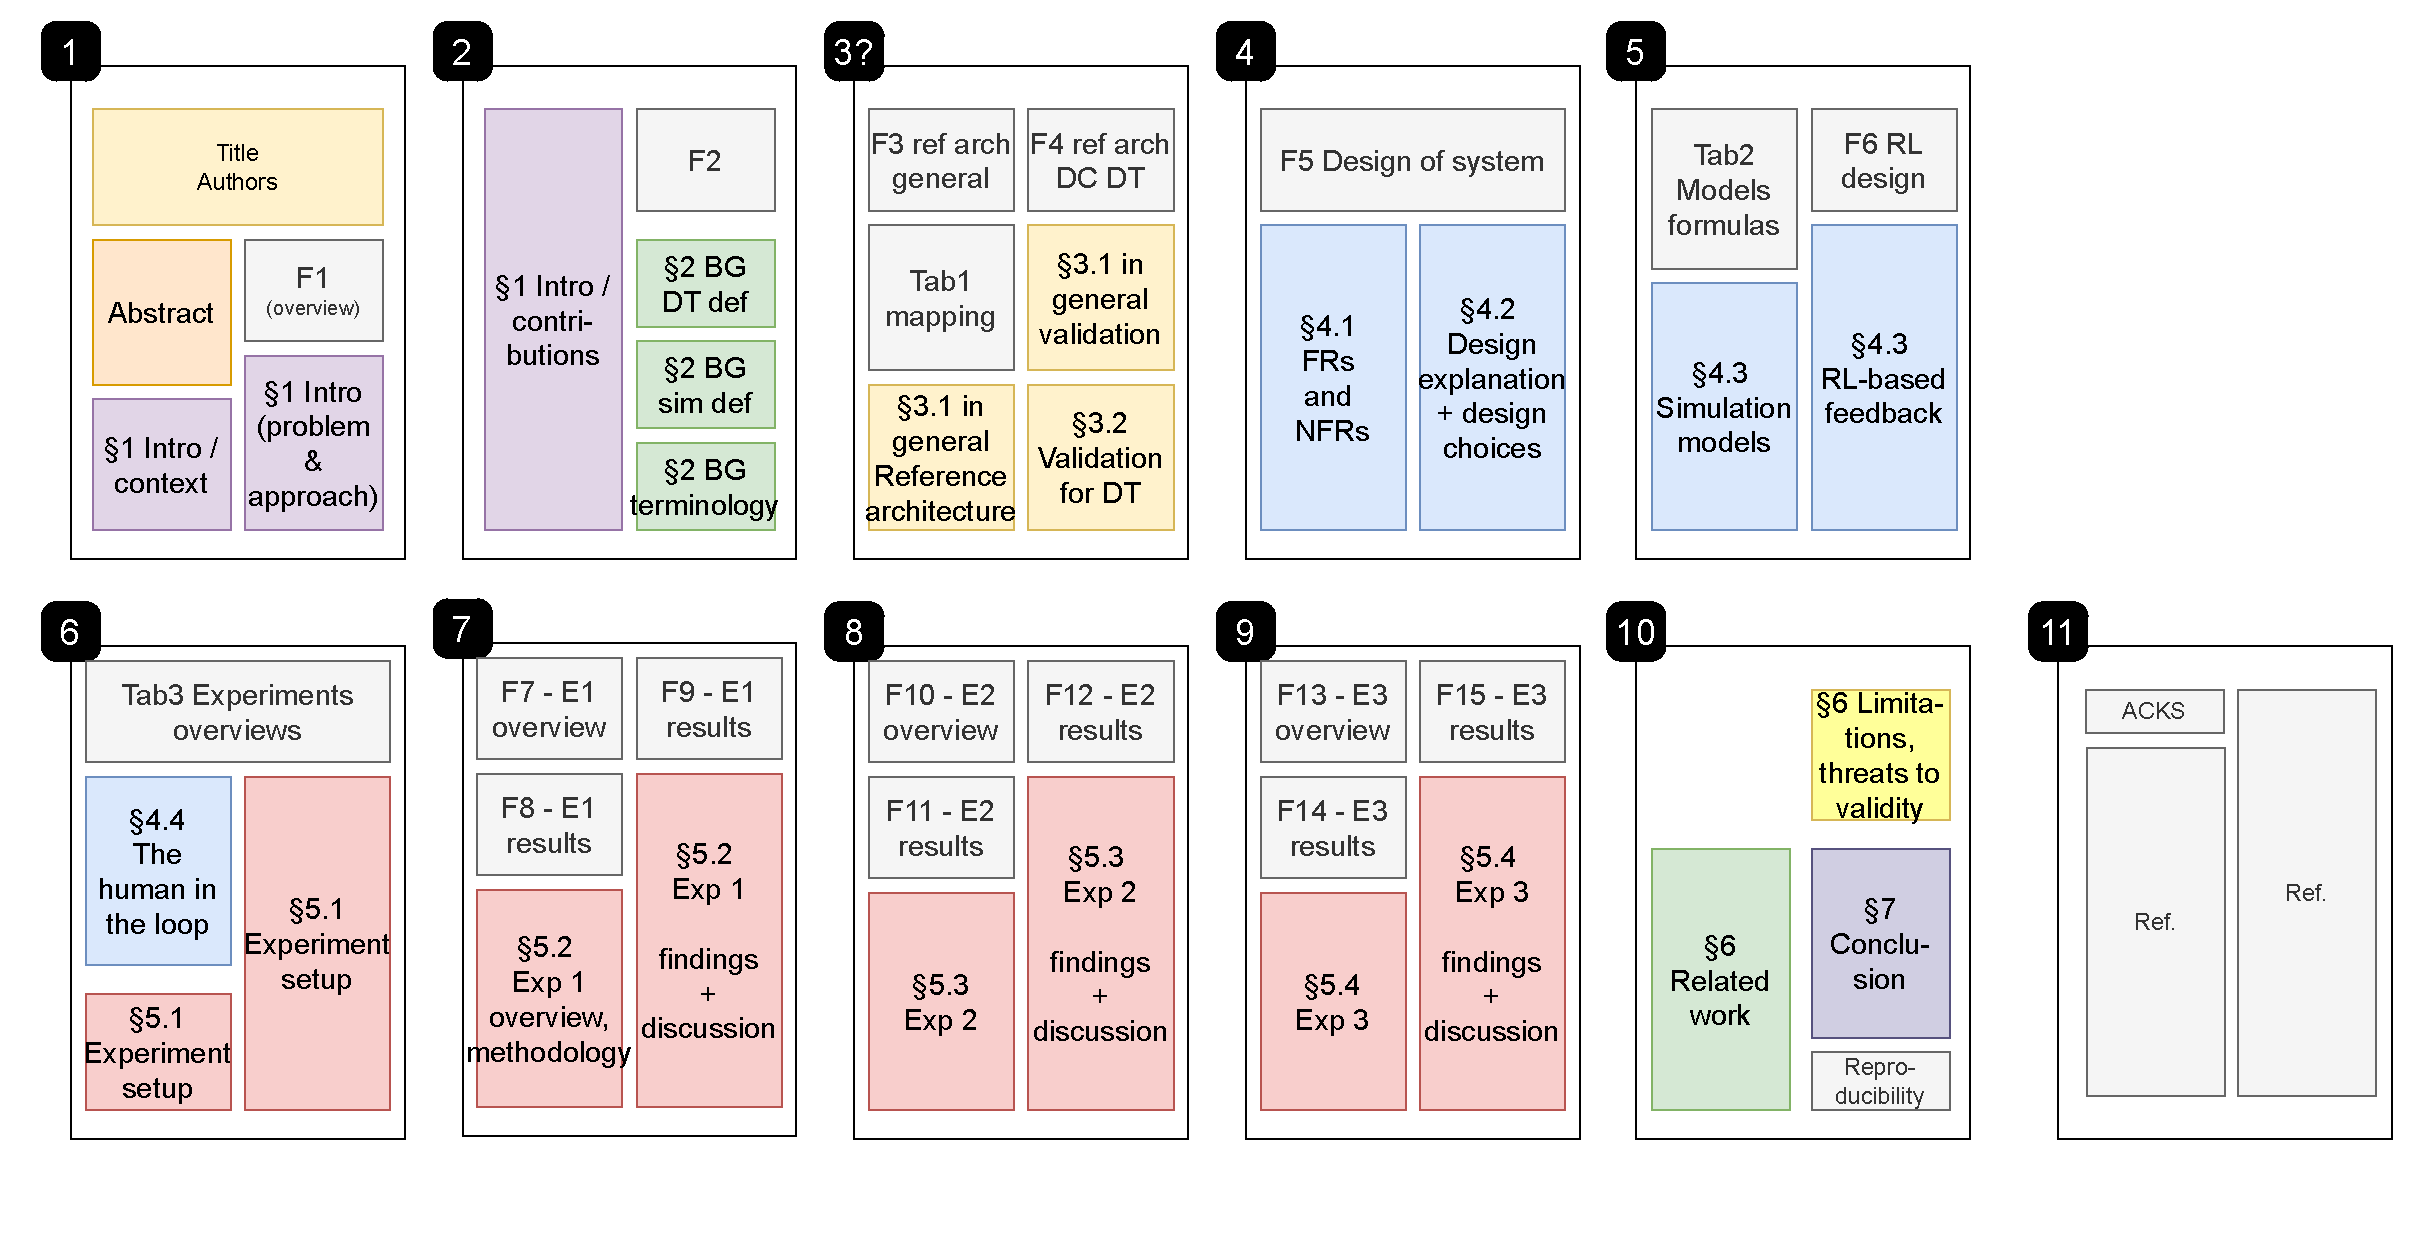
\includegraphics[width=0.99\linewidth]{report/figures/page-budget-digital-twin-engineering.pdf}
    \caption{Caption}
    \label{fig:placeholder}
\end{figure*}

\end{document}
